\section{From UML to SQL}

The transition from a UML-based representation to a relational database structure requires defining attributes within entities that will serve as primary keys for tables and foreign keys referencing the primary keys of associated entities (tables).

\subsection{UML Modeling (Version 1.4)}

Based on the cardinalities of the associations, we can represent primary and foreign keys in the previous UML model (e.g., personne.id, soigneur.personne\_id, etc.).

\begin{figure}[H]
\begin{center}
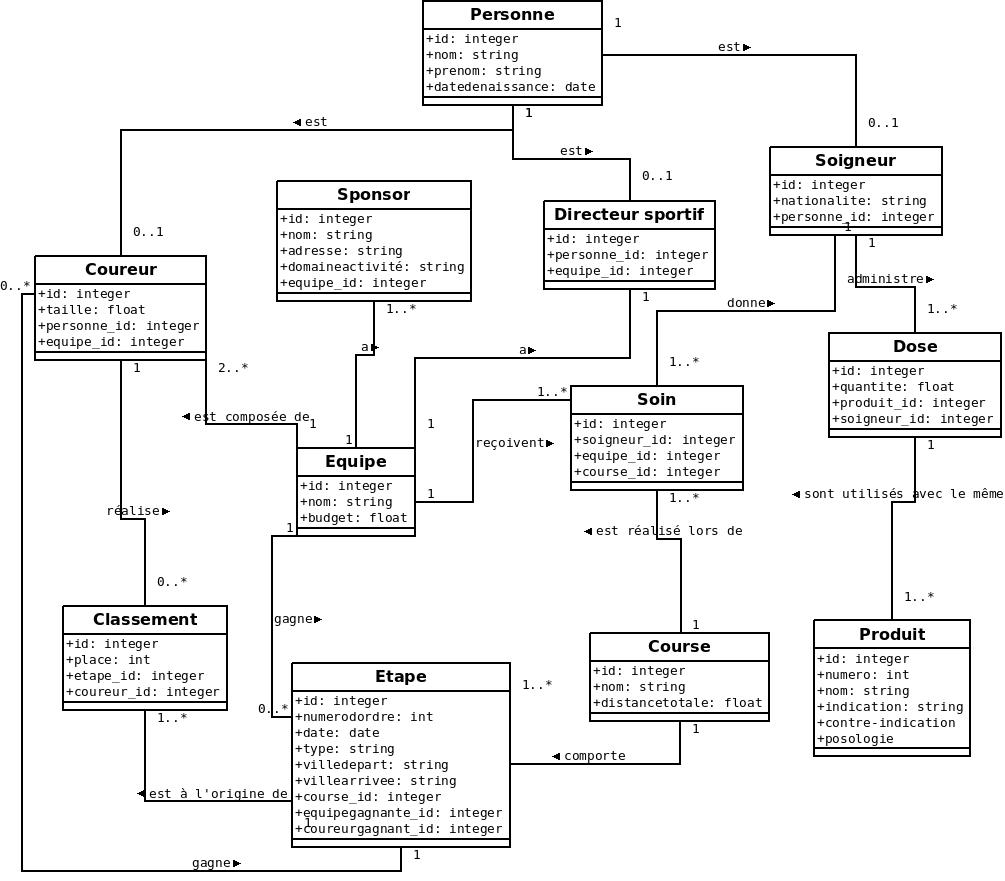
\includegraphics[height=6.5cm]{Figure5.jpg}\\
\caption{Model: Key Attributes}
\label{fig5}
\end{center}
\end{figure}

\subsection{Database Structuring}

From this UML schema, we can implement the database structure in SQL.

\begin{itemize}
\item personne (\underline{id}, nom, prenom, datedenaissance)
\item coureur (\underline{id}, taille, \#personne\_id, \#equipe\_id)
\item sponsor (\underline{id}, nom, adresse, domaineactivité, \#equipe\_id)
\item directeur sportif (\underline{id}, \#personne\_id, \#equipe\_id)
\item soigneur (\underline{id}, nationalite, \#personne\_id)
\item equipe (\underline{id}, nom, budget, \#ds\_id)
\item soin (\underline{\#soigneur\_id, \#equipe\_id, \#course\_id})
\item dose (\underline{\#produit\_id, \#soigneur\_id}, quantite)
\item classement (\underline{id}, place, \#etape\_id, \#coureur\_id)
\item etape (\underline{id}, numerodordre, date, type, villedepart, villearrivee, \#course\_id, \#equipegagnante\_id, \#coureurgagnante\_id)
\item course (\underline{id}, quantite, \#produit\_id, \#soigneur\_id)
\item produit (\underline{id}, quantite, \#produit\_id, \#soigneur\_id)
\end{itemize}

In this representation, primary keys are underlined, and foreign keys are prefixed with a hashtag (\#).  
In SQLite, it is neither necessary nor recommended to define an automatically incremented (AUTOINCREMENT) primary key, as a rowid is directly available.

With this structure, we can create the database.

\lstinputlisting[language=SQL]{sql/key.sql}

The full SQL script for creating all database tables is available in the appendix.

\subsection{Inserting Data into the Database}

With this structure in place, we can populate the database by inserting data and performing updates using SQL commands such as:

\begin{lstlisting}[language=SQL]
INSERT INTO ... VALUES (...);
UPDATE ... SET ... WHERE ...;
\end{lstlisting}

\lstinputlisting[language=SQL]{sql/insert.sql}

% The appendix contains SQL scripts for inserting data into all database tables.  
% Examples of update operations are also provided.

\subsection{Joins: Retrieving Information}

Once the database is properly structured, we must be able to retrieve all necessary information using table joins.  
The SQL query below demonstrates a join across all database tables.  
Column renaming is applied where multiple tables contain attributes with the same name.

\lstinputlisting[language=SQL]{sql/joint.sql}

% The appendix includes additional examples of SQL joins between tables.  
% Views can also be created for specific table joins when necessary.
